\chapter{Blood ejection from a ventricle into aorta}

\modinfo{Test}{ArteryOutlet}
\modinfo{Directory}{ArteryFlow}
\modinfo{Solvers}{\Idx{FlowSolve},\Idx{ElasticSolve}, \Idx{OutletCompute}} 
\modinfo{Tools}{Editor, \Idx{Fortran 90 compiler}, \Idx{ElmerGrid}}
\modinfo{Dimensions}{2D, Transient}

\subsection*{Case description}

This tutorial is about simulating blood ejection in to the elastic human aorta.
The idea is to mimic left ventricle contraction and resulting pulse propagation 
in an elastic conduit. In the simulation about 0.8 
deciliters of blood is ejected to a 50 cm long elastic aorta during a time 
period of 400 ms.  In order to get the outlet of the model behave 
physiologically more realistic way, a one dimensional model is coupled
with the higher order model.
 
\subsection*{Solution procedure}

First we generate the mesh of 366 eight-node quadrilaterals elements with 
the command
\ttbegin
ElmerGrid 1 2 contra
\ttend
Next we generate one dimensional mesh to the outlet of the 2D model.
The program {\tt AddOneDim} is posed to be run in the mesh directory
{\tt contra}.  The length, the number of the elements, 
and the coordinate direction of the 1D section will be asked.

In the simulation block the timestep is set equal to 1 ms and 
total simulation time equal to 600 ms.  The geometry consists of five bodies
of which the first three are for the fluid volume.  Body number 1 os the 
contracting volume.  Body 2 is a short rigid channel between the body 1 and 
the elastic artery. Artificial compressibility
method is used for the fluid volume (body 3) which is in contact with the 
elastic wall (body 4).  One dimensional model is the body 5. 
Material settings for those are 
following:
\ttbegin
! Bodies 1 and 2 (blood)
Material 1
  Density = 1000
  Viscosity = 3.5e-3
  Youngs Modulus = 1
  Poisson Ratio = 0.3
End

! Body 3 (blood)
Material 2
  Density = 1000
  Viscosity = 3.5e-3
  Youngs Modulus = 1
  Poisson Ratio = 0.3
  Compressibility Model = Artificial Compressible
  Artificial Compressibility  = 3.3E-5 
End

! Body 4 (elastic wall)
Material 3
  Density = 1010
  Youngs Modulus = 3.0e5
  Poisson Ratio = 0.45
End

! One dimensional model
Material 4
   Density = 1010.0
   Artery Wall Youngs Modulus = Real 3.0e5 
   Artery Radius = Real 0.0135 
   Artery Wall Thickness = Real 0.002
   Artery Poisson Ratio  = Real 0.45
End
\ttend

Notice that the radius of the one dimensional model ({\tt Artery Radius})
is to the midplane of the wall (inner radius + half of the wall thickness).
The overall FSI iteration scheme is started by one dimensional solver
({\tt OutletCompute}, see the solver manual), after that Navier-Stokes, 
elasticity and mesh update solvers are run.  Steady state convergence tolerance
is set equalt to 1.0E-4 for each of the solvers.  The nonlinearities
of each of the solvers are computed within the FSI scheme loop, that is,
the flag {\tt Nonlinear System Max Iterations} is set equal to 1.
Artificial compressibility coefficient is computed by the equation
$c = (1-\nu^2) [D/(E~h)]$, where $\nu$ is the Poisson ratio of the
artery wall, $D$, $E$ and $h$ are the inner diameter, Young's modulus
and the thickness of the artery, respectively.

The only driving force of the system, the wall motion of the contracting 
fluid domain is given by the fortran function {\tt Motion}, see the
figure \ref{fig:contra}.  The boundary condition setting is
\ttbegin
! Moving boundary
Boundary Condition 1
  Target Boundaries = 1
  Velocity 1 = 0
  Velocity 2 = Equals Mesh Velocity 2
  Mesh Update 1 = Real 0
  Mesh Update 2 = Variable Time
       Real Procedure "./Motion" "Motion"
End
\ttend

At the outlet, the pressure boundary condition is given by the
function {\tt OutletPres} and the corresponding radial displacement
of the end wall of the outlet is given by the function {\tt OutletdX}
\ttbegin
! Outlet pressure of the 2D model
Boundary Condition 2
  Target Boundaries = 2
  Flux Integrate = Logical True
  Flow Force BC = True
  Pressure 2 = Variable Time
      Real Procedure "./ArteryOutlet" "OutletPres"
  Mesh Update 2 = Real 0
End

! Radial displacement of the end wall at the outlet of 2D model
Boundary Condition 9
  Target Boundaries = 9
  Displacement 1 = Variable Time
      Real Procedure "ArteryOutlet" "OutletdX"
  Displacement 2 = 0 
End
\ttend
FSI interface boundary is described as following
\ttbegin
! FSI interface boundary
Boundary Condition 11
  Target Boundaries = 11
  Velocity 1 = Equals Mesh Velocity 1
  Velocity 2 = Equals Mesh Velocity 2
  Mesh Update 1 = Equals Displacement 1
  Mesh Update 2 = Equals Displacement 2
  Force BC = Logical True
End
\ttend
Finally, the coupling of the 1D model with the 2D is 
done at the inlet boundary as
\ttbegin
Boundary Condition 16
  Target Boundaries = 16
  Fluid Coupling With Boundary = Integer 2
  Structure Coupling With Boundary = Integer 9
End
\ttend


\subsection*{Results}

The contraction is curve seen in the figure \ref{fig:contra} and
the velocity fields at different time levels are presented
in the figure~\ref{fig:velofields}.  Postprocessing instructions
are given in the file {\tt PostProcessingInstr.txt}.

\begin{figure}[!hb]
\begin{center}
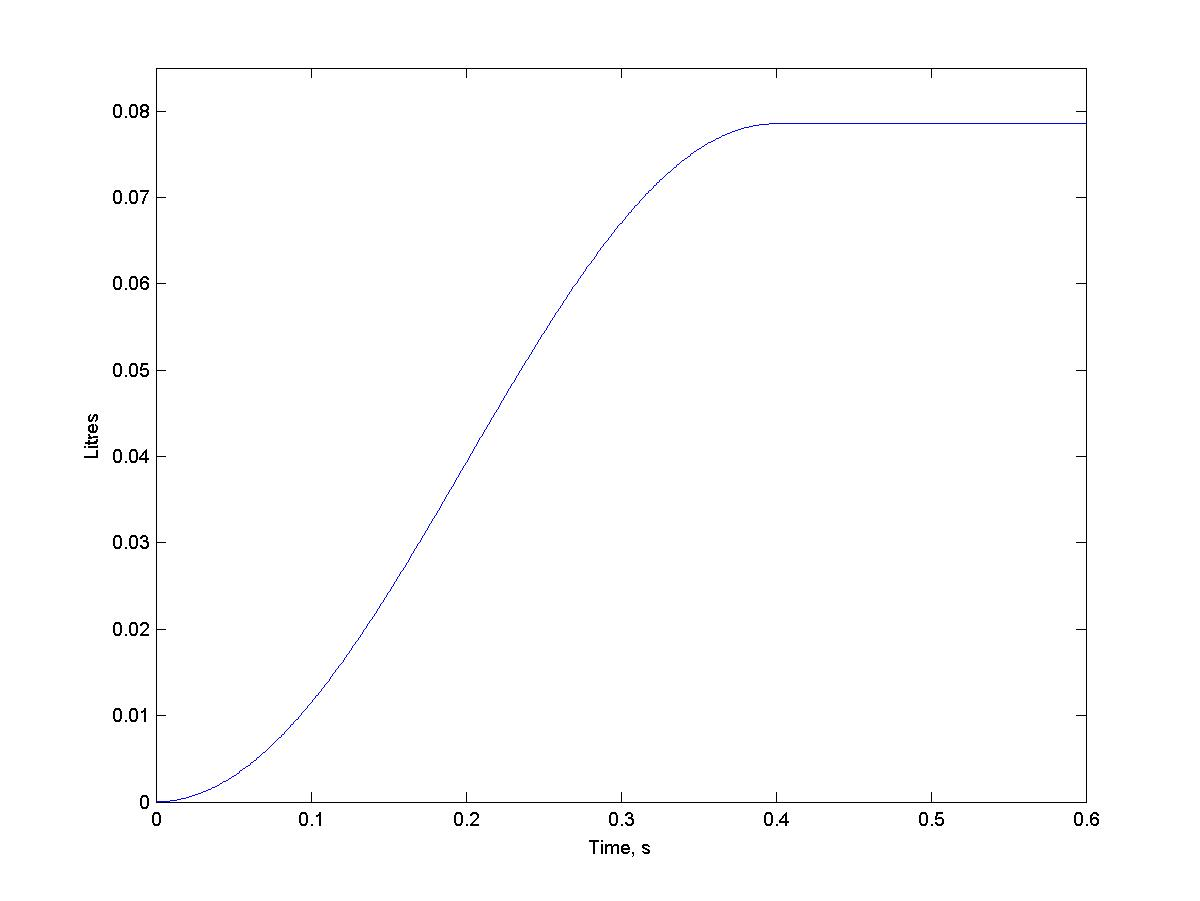
\includegraphics[width=15cm]{motion}
\caption{Contraction curve generated by the function {\tt Motion}.}
\label{fig:contra}
\end{center}
\end{figure}

\begin{figure}[!hb]
\begin{center}
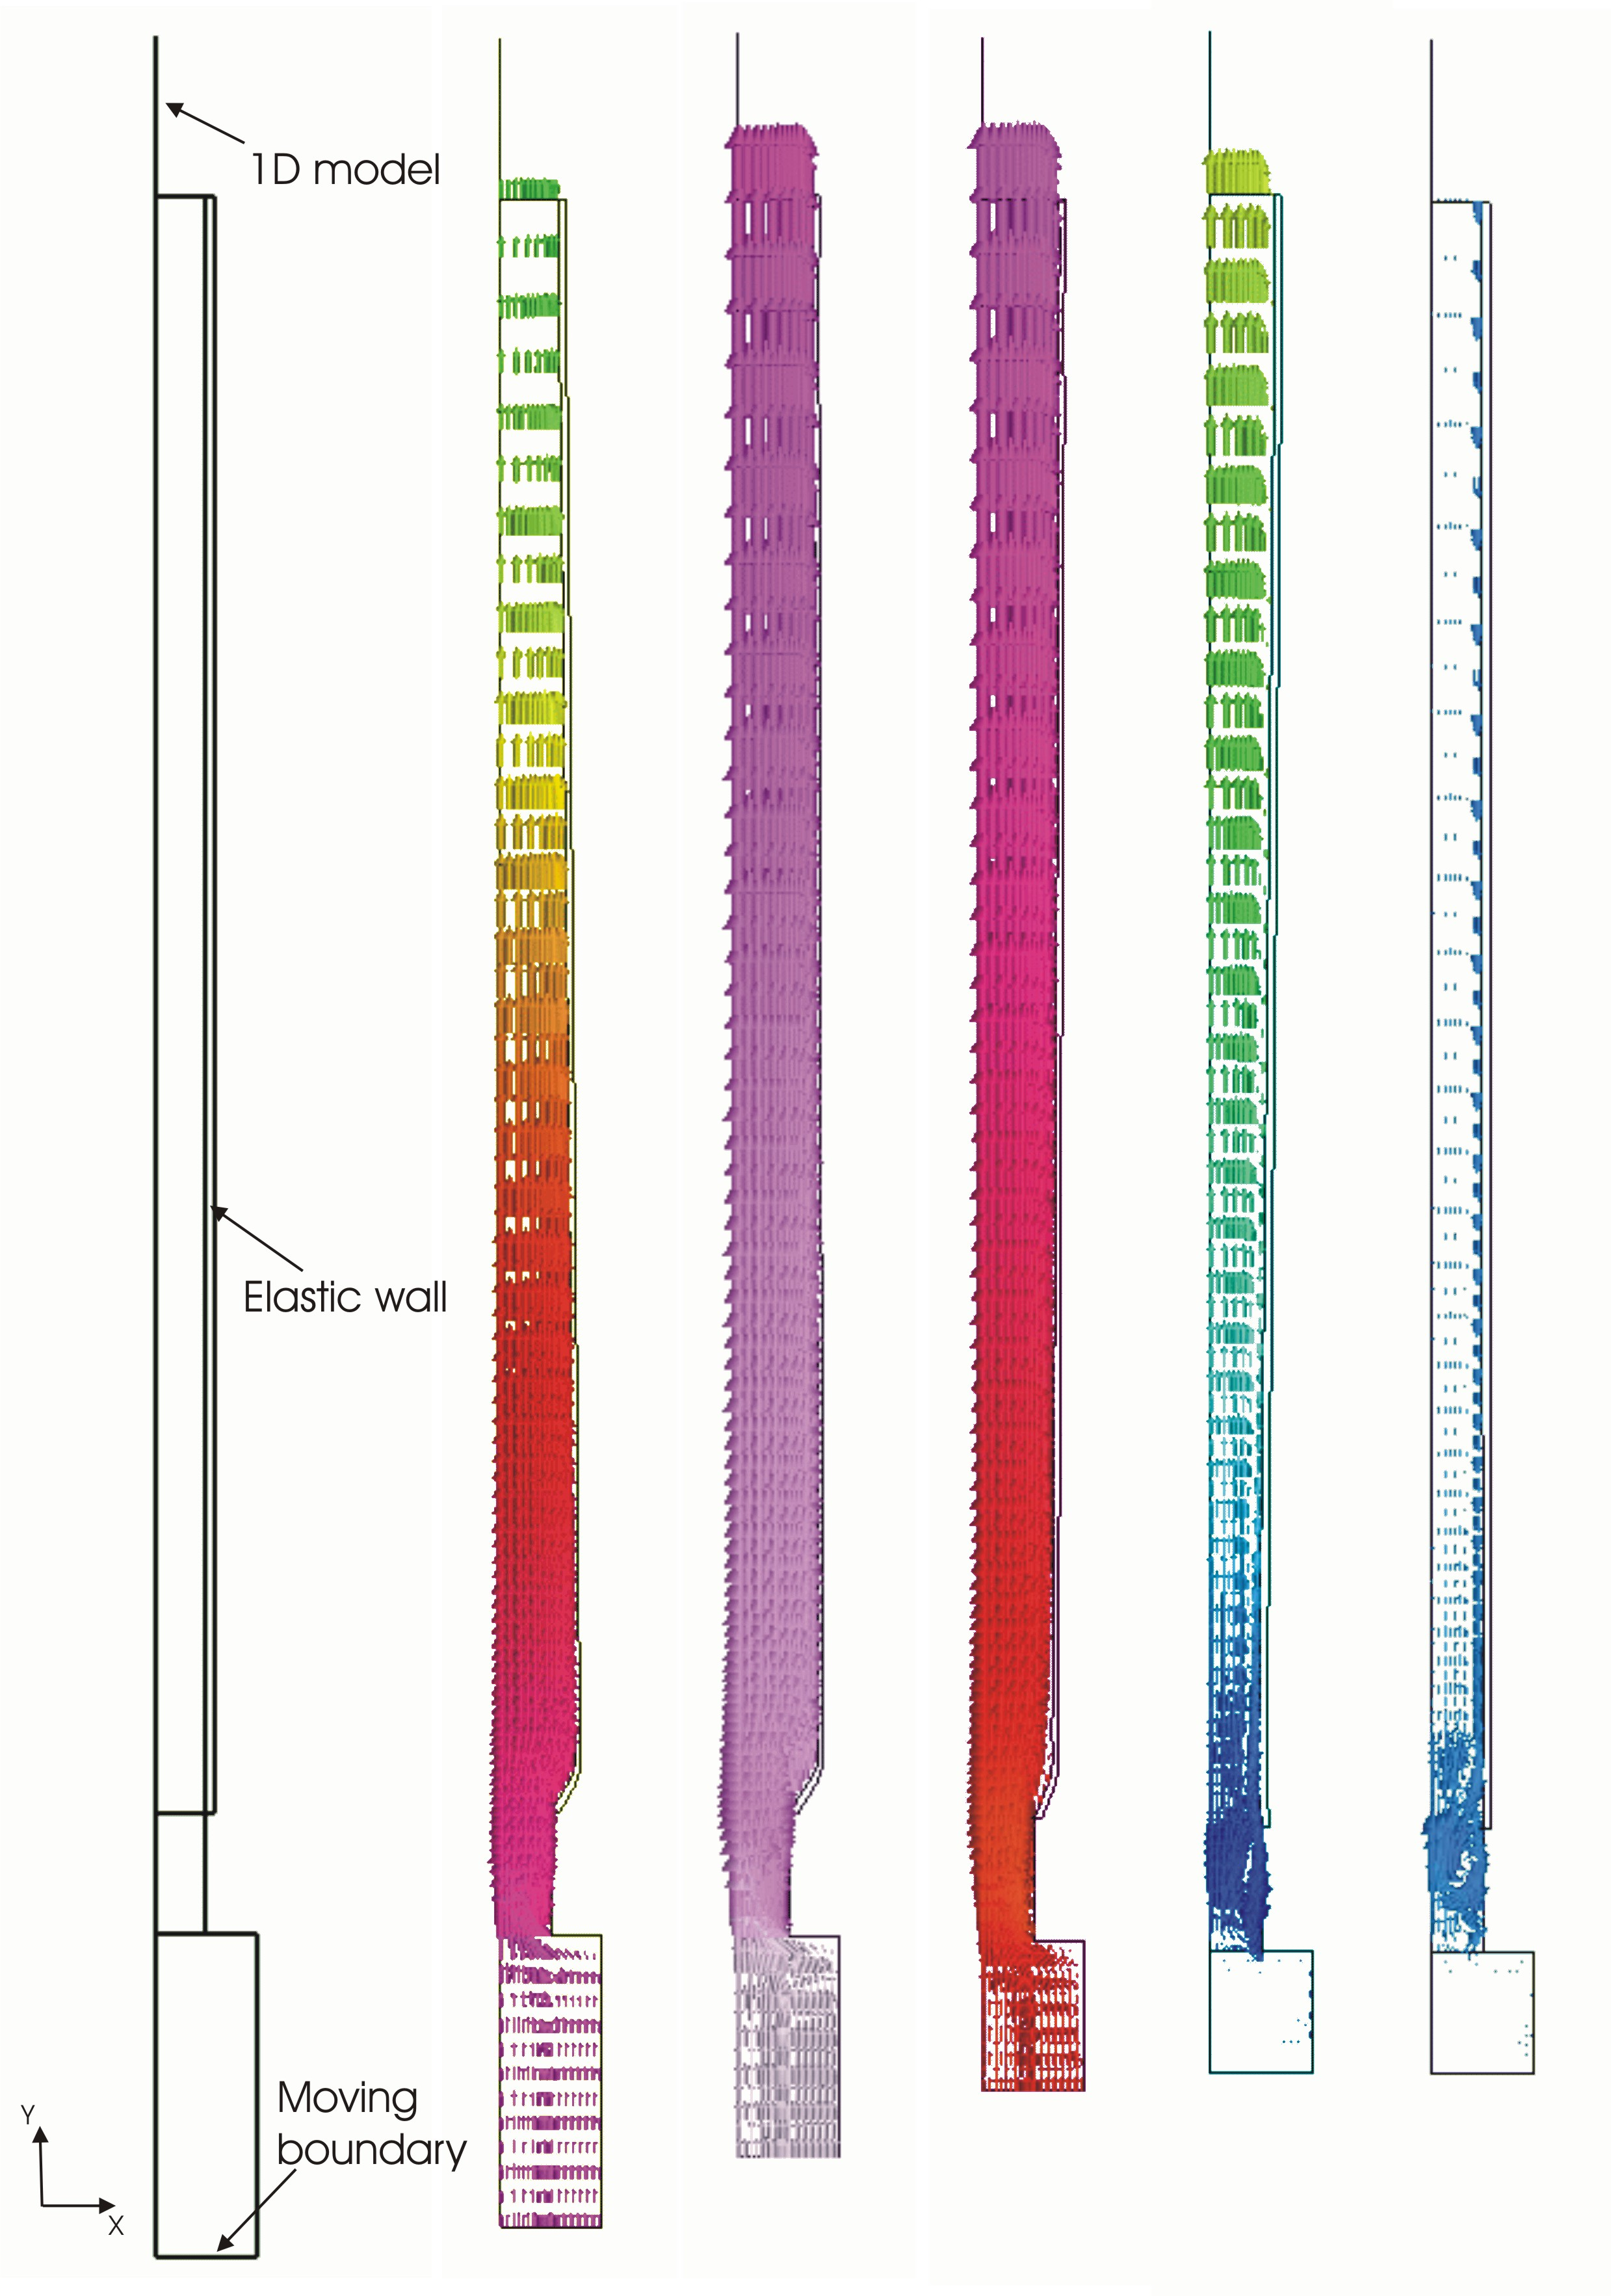
\includegraphics[width=\textwidth]{collage}
\caption{The geometry of the model and velocity fields at 5 time steps, 
100, 200, 300, 400 and 500 ms.  The displacements of the wall are 
magnified by factor of 10.}
\label{fig:velofields}
\end{center}
\end{figure}

